\scanpage{17}

\deleted{\diagram{\begin{tikzcd}[ampersand replacement=\&,column sep=small,row sep=large]
\& \vec S(\unsure{X_0|X_\bullet})\simeq G_0 \arrow[dl] \arrow[d] \arrow[dr] \& \\
S(X_0)\simeq G_0/H_S \& A(X_0)\simeq G_0/H_A, \& F(X_0)\simeq G_0/H_F
\end{tikzcd}}}

\deleted{\[
H_S\cap H_A=e,\qquad H_A\cap H_F=e,\qquad H_S\cap H_F=e
\]}

\deleted{\unsure{i.e.|among others}
\[
G_0\hookrightarrow G_0/H_S\times G_0/H_A,\qquad
G_0\hookrightarrow G_0/H_A\times G_0/H_F,\qquad
G_0\unsure{\hookrightarrow|\subset}\deleted{\unsure{G_0|H_S}}/H_A\times G_0/H_F
\]}

\deleted{\figure{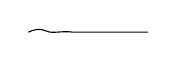
\begin{tikzpicture}[x=1cm,y=1cm]
\draw (0,0).. controls (.1,.04) and (.14,.05) .. (.24,.01).. controls (.31,-.02) and (.43,.02) .. (.57,0)--(1.52,0);
\end{tikzpicture}}}

\margin{\uline{\unsure{Unoriented case}}}

\deleted{Let us consider the category of polyhedra (unoriented) of given type; there are functors}

\deleted{\[
\begin{array}{l}
S\\
\vec A\\
F\\
\deleted{\unsure{A|R}}
\end{array}
\]}

\deleted{\diagram{\(\begin{array}{lll}
A_1 & \text{incidence relation between }S\text{ and }A & \text{(}\unsure{\text{oriented edges}}\text{ in sense }1\text{)}\\
A_2 & \rule{3.2cm}{0.25pt}\ A\text{ and }F & (\rule{2.8cm}{0.25pt}\ 2)\\
A_3 & \text{incidence relation between }\unsure{S|B}\text{ and }F &
\end{array}\)}}

\deleted{\[
R=\deleted{\unsure{A_3}}\unsure{\simeq|=}A_1\times_A A_2
\]
\deleted{\unsure{relation} of incidence between $S$ and $F$}
\inserted{\unsure{triples or flags|triples of flags} $(s,a,f)$\quad$s\unsure{\leq|<}a<f$.}}

\deleted{\diagram{\begin{tikzcd}[ampersand replacement=\&,row sep=small,column sep=small]
\& R \arrow[dl] \arrow[d] \arrow[dr] \& \\
S\&A\&F
\end{tikzcd}}}

\deleted{\[
\begin{aligned}
A_1&=\operatorname{Im}(R\to S\times A)\\
A_2&=\operatorname{Im}(R\to A\times F)\\
A_3&=\operatorname{Im}(R\to S\times F)
\end{aligned}
\]}

\deleted{$\Omega$ set of orientations}

\deleted{\[
{A_1}_{\Omega}\simeq\unsure{{A_2}_{\Omega}}\simeq{A_3}_{\Omega}\qquad(
\]}

\[
\mathrm{Pol}_{\unsure{\tau|t}}\qquad
\mathrm{Pol}_{\tau}^{\unsure{\mathrm{or}}}\simeq
\mathrm{Pol}_{\tau}\deleted{\unsure{/\Omega}}\inserted{{}_{/\Omega}}
\]

\margin{16}

\scanpage{18}
\mspage{6}

$S\mathcal T_{1,1}\simeq$ \unsure{inverse image} of $\mathrm S\ell(2,\mathbb Z)$ in $\unsure{\deleted{\mathrm G\ell}\mathrm S\ell(2,\mathbb R)^{\sim}|\mathrm G\ell(2,\mathbb R)^{\sim}}$
\[
\simeq\{\rho,\sigma\mid\rho^3=\sigma^2\ (=\omega)\}
\]
\margin{\unsure{(}central \unsure{elem\textsuperscript{ent}|el\textsuperscript{ement}}}

\[
\mathcal T_{11}=S\mathcal T_{11}/\langle\omega^2\rangle
\]

\[
\begin{array}{ll}
(\mathcal T_{11})_{\mathrm{ab}}\simeq\mathbb Z & (\mathcal T_{11})_{\mathrm{ab}}\simeq\mathbb Z/12\mathbb Z\\[4pt]
\deleted{(\rho,\sigma)} & \\
\rho\longmapsto2 & \rho\longmapsto2\bmod12\\
\sigma\longmapsto3 & \sigma\longmapsto3\bmod12\\
\omega\longmapsto\unsure{6|8} &
\end{array}
\]

\diagram{\begin{tikzcd}[ampersand replacement=\&,row sep=large,column sep=small]
\& 1 \& \& 1 \\
\& \mathcal T_{11} \arrow[u] \arrow[r] \& \deleted{\unsure{\mathcal T_{\mathrm{ab}}}} \arrow[r] \& \mathbb Z/12\mathbb Z \arrow[u] \\
\unsure{\widetilde\omega|\bar\omega}=\omega^{2\deleted{\unsure{4}}} \& S\mathcal T_{11} \arrow[u] \arrow[rr] \arrow[ur,phantom,"\deleted{\text{cartesian}}"{description}] \& \& \mathbb Z \arrow[u] \\
\uline{1} \arrow[u] \& \mathbb Z \arrow[u] \arrow[rr,"\mathrm{id}"] \& \& \mathbb Z \arrow[u,"12"] \\
\& 1 \arrow[u] \& \& 1 \arrow[u]
\end{tikzcd}}

\margin{so $S\mathcal T_{11}$ is obtained from $\mathcal T_{11}$ by inverse image of the canonical extension of $\mathbb Z/12\mathbb Z$ by $\mathbb Z$, via $\mathcal T_{11}\to\mathbb Z/12\mathbb Z$.}

\deleted{a normalization of $(K,\unsure{K_0|N|k_0})$, \unsure{then} it is \unsure{special} : the category of étale coverings in $\unsure{K'_fN|K'_{fN}}$ -- \deleted{\illegible{1}} $\Delta$ \unsure{covering|i.e.} $\Delta$ topological \unsure{has} a unique normalization for which the projection \unsure{is|be} a \unsure{morphism} of \unsure{normalized} $\Delta$-complexes. [But beware, \unsure{it works} \uline{\unsure{not}} for \unsure{strict normalizations} \unsure{even|necessarily}\ldots]}

\deleted{\unsure{8.|$\beta$.} \unsure{Fundamental|Fundamental} \unsure{groups|group} and groupoids. We \unsure{shall show|show} the relation between topological construction and algebraic construction.}

\margin{17}

\scanpage{19}

% pencil numeral at the top right corner; no other foliation numeral is visible on this sheet
\margin{8v}

\figure{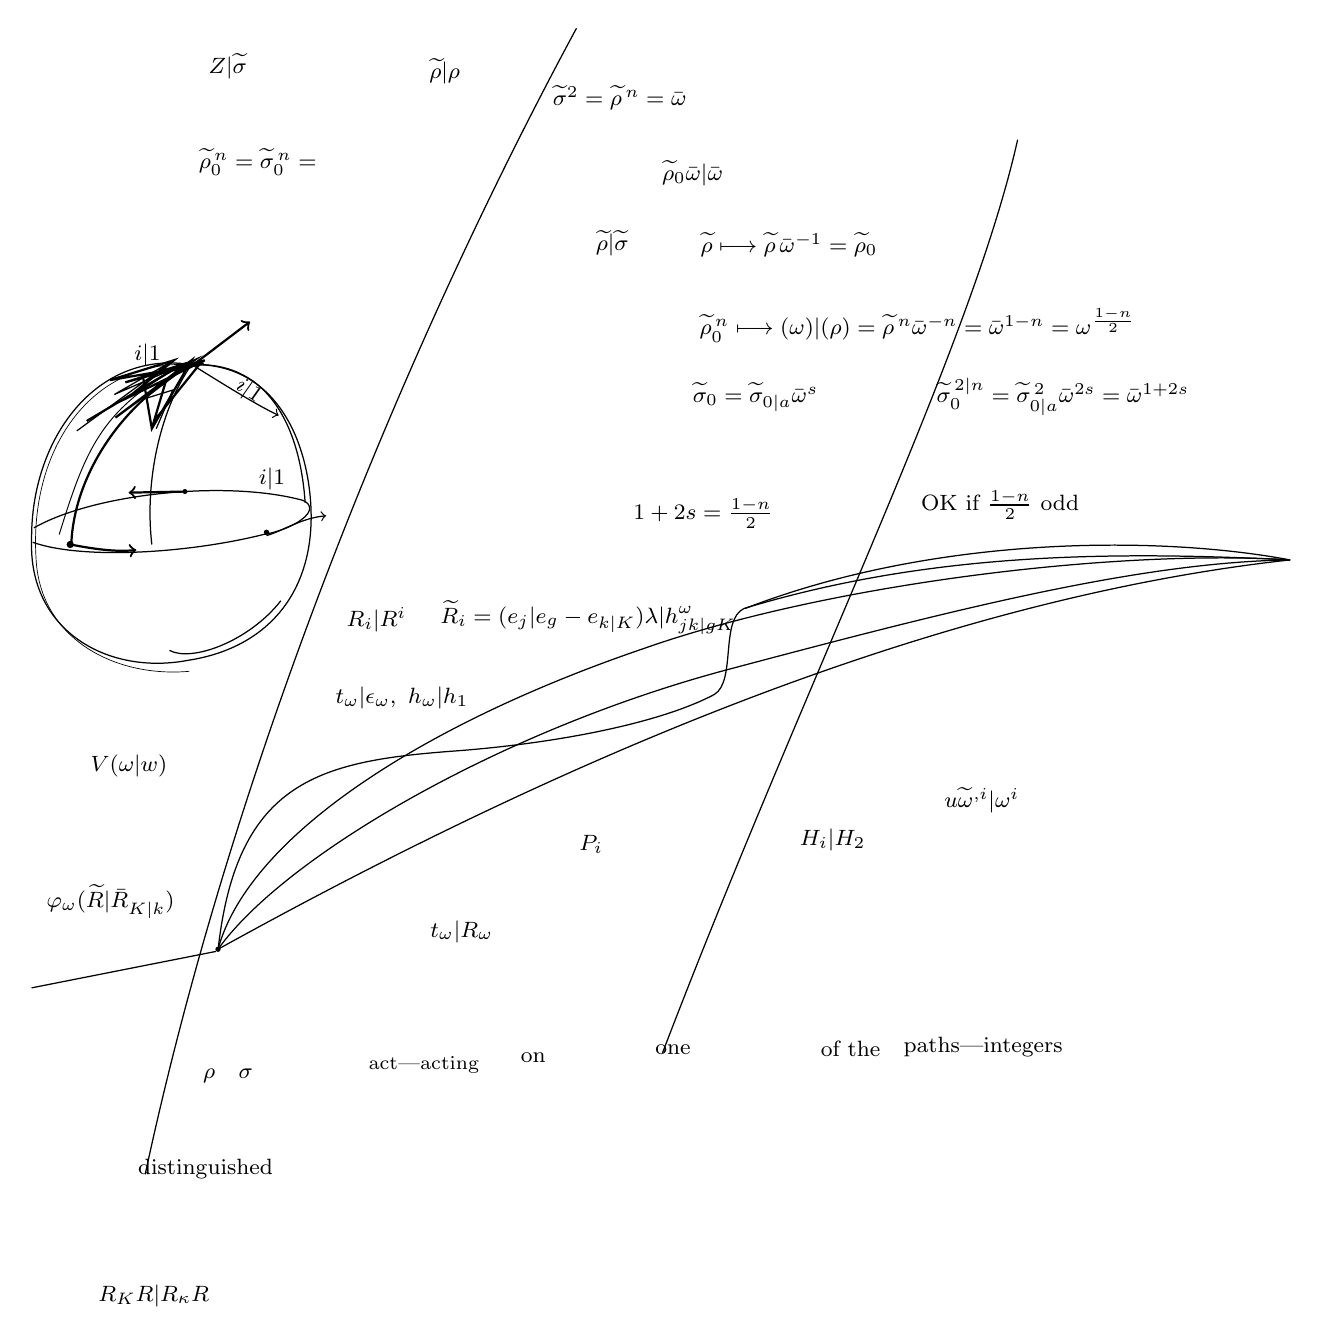
\begin{tikzpicture}[x=.014cm,y=-.014cm,every node/.style={font=\footnotesize,inner sep=0pt},line width=.45pt]
\node[anchor=west] at (385,80) {$\deleted{\unsure{\mathbb Z|\widetilde\sigma}}$};
\node[anchor=west] at (585,85) {$\deleted{\unsure{\widetilde\rho|\rho}}$};
\node[anchor=west] at (376,167) {$\widetilde\rho_0^{\,n}=\widetilde\sigma_0^{\,n}=$};
\node[anchor=west] at (697,109) {$\widetilde\sigma^2=\widetilde\rho^{\,n}=\bar\omega$};
\node[anchor=west] at (796,177) {$\deleted{\unsure{\widetilde\rho_0\bar\omega|\bar\omega}}$};
\node[anchor=west] at (736,241) {$\deleted{\unsure{\widetilde\rho|\widetilde\sigma}}$};
\node[anchor=west] at (831,242) {$\widetilde\rho\longmapsto\widetilde\rho\,\bar\omega^{-1}=\widetilde\rho_0$};
\node[anchor=west] at (830,315) {$\widetilde\rho_0^{\,n}\longmapsto\deleted{\unsure{(\omega)|(\rho)}}=\widetilde\rho^{\,n}\bar\omega^{-n}=\bar\omega^{1-n}=\omega^{\frac{1-n}{2}}$};
\node[anchor=west] at (824,380) {$\widetilde\sigma_0=\widetilde\sigma_{\unsure{0|a}}\bar\omega^s$};
\node[anchor=west] at (1045,380) {$\widetilde\sigma_0^{\,\unsure{2|n}}=\widetilde\sigma_{\unsure{0|a}}^{\,2}\bar\omega^{2s}=\bar\omega^{1+2s}$};
\node[anchor=west] at (770,486) {$1+2s=\frac{1-n}{2}$};
\node[anchor=west] at (1031,478) {OK if $\frac{1-n}{2}$ \uline{odd}};

\draw (328,1085) .. controls (405,726) and (557,346) .. (719,46);
\draw (797,975) .. controls (925,640) and (1077,335) .. (1119,147);

\draw (370,351) .. controls (284,337) and (224,418) .. (225,510) .. controls (222,592) and (294,633) .. (367,619) .. controls (445,607) and (487,549) .. (477,465) .. controls (469,399) and (433,349) .. (370,351);
\draw[line width=.25pt] (371,351) .. controls (277,345) and (223,430) .. (229,526) .. controls (232,599) and (300,635) .. (368,629);
\draw (350,610) .. controls (370,621) and (422,602) .. (451,565);
\draw (227,499) .. controls (281,468) and (401,455) .. (471,474) .. controls (490,483) and (461,501) .. (435,505) .. controls (367,522) and (271,528) .. (226,512);
\draw[line width=.8pt,->] (260,514) .. controls (281,518) and (301,521) .. (320,519);
\draw[line width=.8pt,->] (366,466)--(313,467);
\draw[->] (438,506) .. controls (454,501) and (470,490) .. (492,488);
\fill (260,514) circle[radius=3.3];
\fill (438,503) circle[radius=2.5];
\fill (364,466) circle[radius=2.3];
\draw (334,514) .. controls (327,454) and (343,389) .. (370,351);
\draw[line width=.8pt] (261,514) .. controls (263,455) and (303,388) .. (370,351);
\draw[line width=.35pt] (250,505) .. controls (274,428) and (288,390) .. (365,350);
\draw[line width=.8pt,->] (369,353)--(423,312);
\draw[->] (372,352) .. controls (398,368) and (428,387) .. (449,397);
\draw (377,351) .. controls (437,351) and (468,403) .. (473,476);
\node at (330,342) {$\unsure{i|1}$};
\node[rotate=-35] at (422,375) {$\unsure{i|1}$};
\node at (443,455) {$\unsure{i|1}$};
\draw[line width=.8pt] (275,402)--(361,351)--(310,367)--(382,347)--(312,381)--(354,347)--(296,365)--(377,351)--(336,402)--(347,365)--(301,399)--(370,347)--(334,409)--(326,362)--(381,350);
\draw (266,411)--(352,348)--(300,378)--(376,345)--(327,382)--(353,374)--(338,409);

\node[anchor=west] at (510,582) {$\unsure{R_i|R^i}$};
\node[anchor=west] at (595,580) {$\widetilde R_{\unsure{i}}=(\unsure{e_j|e_g}-e_{\unsure{k|K}})\unsure{\lambda|h}^{\omega}_{\unsure{jk|gK}}$};
\node[anchor=west] at (500,653) {$\unsure{t_\omega|\epsilon_\omega},\ \unsure{h_\omega|h_1}$};
\node[anchor=west] at (278,715) {$V(\unsure{\omega|w})$};
\node[anchor=west] at (238,838) {$\varphi_\omega(\unsure{\widetilde R|\bar R}_{\unsure{K|k}})$};
\node[anchor=west] at (721,786) {$P_i$};
\node[anchor=west] at (586,865) {$\deleted{\unsure{t_\omega|R_\omega}}$};
\node[anchor=west] at (921,782) {$\deleted{\unsure{H_i|H_2}}$};
\node[anchor=west] at (1052,746) {$u\unsure{\widetilde\omega^{,i}|\omega^i}$};

\draw (225,916)--(392,883);
\fill (394,881) circle[radius=2.4];
\draw (394,882) .. controls (411,727) and (487,710) .. (612,701) .. controls (702,694) and (795,676) .. (844,650) .. controls (864,638) and (849,582) .. (871,572) .. controls (1039,521) and (1205,520) .. (1366,528);
\draw (394,881) .. controls (422,778) and (581,676) .. (781,608) .. controls (949,549) and (1211,518) .. (1366,528);
\draw (394,881) .. controls (454,797) and (649,683) .. (854,628) .. controls (1057,574) and (1228,530) .. (1366,528);
\draw (394,881) .. controls (721,700) and (1056,562) .. (1366,528);
\draw (872,572) .. controls (1045,505) and (1249,506) .. (1366,528);

\node[anchor=west] at (380,996) {$\rho\quad\sigma$};
\node[anchor=west,font=\scriptsize] at (530,986) {\unsure{act|acting}};
\node[anchor=west] at (668,979) {on};
\node[anchor=west] at (790,972) {one};
\node[anchor=west] at (940,971) {of the};
\node[anchor=west] at (1015,970) {\unsure{paths|integers}};
\node[anchor=west] at (321,1080) {distinguished};
\node[anchor=west] at (285,1195) {$\deleted{\unsure{R_KR|R_\kappa R}}$};
\end{tikzpicture}}